\documentclass[12pt]{article}

% Modelo de artigos da Sociedade Brasileira de Computacao (SBC).
\makeatletter
\def\input@path{{latex/}}
\makeatother
\usepackage{sbc-template}
\usepackage{graphicx,url}
\usepackage[T1]{fontenc}
\usepackage[utf8]{inputenc}
\usepackage[brazil]{babel}
\usepackage{amsmath}
\usepackage{array}
\usepackage{flafter}
\usepackage{float}
\usepackage{placeins}

% Deixa os floats ocuparem mais da página e reduz páginas só com figuras.
\renewcommand{\topfraction}{0.92}
\renewcommand{\bottomfraction}{0.85}
\renewcommand{\textfraction}{0.06}
\renewcommand{\floatpagefraction}{0.75}

\sloppy

\DeclareRobustCommand{\artefato}[1]{\url{#1}}
\newcommand{\pendente}[1]{\textbf{[PENDENTE: #1]}}

\title{BrainSniffer: protótipo reproduzível para estimar uma referência BIS a partir de EEG frontal}

\author{Bruno Rocha Guimarães\inst{1}}

\address{Ciência da Computação -- Centro Universitário Jorge Amado\\
  Salvador, Bahia -- Brasil}

\begin{document}

\maketitle

\begin{abstract}
This paper describes BrainSniffer, a reproducible engineering prototype that estimates a Bispectral Index (BIS) reference label from frontal electroencephalography (EEG). The pipeline uses five-second windows at 128 Hz, a compact one-dimensional convolutional neural network, and partitions grouped by case or subject. The active Figshare-only checkpoint reached mean absolute error (MAE) 7.03 and Pearson correlation 0.784 in a five-case Figshare holdout, but 12.43 and 0.024 in a 15-case VitalDB cross-dataset assessment. A mixed candidate trained with Figshare and part of VitalDB reached 6.69/0.818 on the Figshare benchmark and 8.60/0.688 on the historical VitalDB participant holdout. These results are retrospective and exploratory; Pearson is interpreted as association, not agreement. BrainSniffer neither measures consciousness nor supports clinical decisions, alarms, or drug dosing. Implementation and results are documented in internal artifacts \cite{brainsnifferArtefatos}.
\end{abstract}

\begin{resumo}
Este artigo descreve o BrainSniffer, protótipo de engenharia reproduzível que estima, a partir de eletroencefalografia (EEG) frontal, um rótulo de referência do Índice Bispectral (BIS). O pipeline usa janelas de cinco segundos a 128 Hz, uma rede neural convolucional unidimensional compacta (\textit{compact 1-D CNN}, \texttt{Conv1DDepthEstimator}) e partições agrupadas por caso ou pessoa. O checkpoint ativo, treinado apenas no Figshare, obteve erro absoluto médio (MAE) 7,03 e correlação de Pearson 0,784 em cinco casos Figshare, mas 12,43 e 0,024 em uma avaliação cruzada com 15 casos VitalDB. Um candidato misto, treinado com Figshare e parte do VitalDB, obteve 6,69/0,818 no benchmark Figshare e 8,60/0,688 no holdout histórico VitalDB por participante. Os resultados são retrospectivos e exploratórios; Pearson é tratado como associação, não acordo. O BrainSniffer não mede consciência nem apoia decisão clínica, alarme ou dose. Implementação e resultados constam de artefatos internos \cite{brainsnifferArtefatos}.

\textbf{Palavras-chave:} EEG frontal; rótulo BIS; CNN 1-D; validação agrupada; mudança de domínio; reprodutibilidade.
\end{resumo}

\section{Introdução}

O Índice Bispectral (Bispectral Index, BIS) é uma saída proprietária calculada a partir da eletroencefalografia (EEG), o registro da atividade elétrica cerebral captada no couro cabeludo. Sua escala vai de 0, próximo de silêncio elétrico, a 100, tipicamente associado à vigília, e a faixa intermediária costuma ser usada como referência de hipnose em anestesia geral, sem que isso defina um limiar clínico único ou uma fronteira nítida entre estados. O cálculo combina características no domínio do tempo e da frequência (incluindo componentes bispectrais e de supressão de surto) por uma regra de combinação não publicada; por ser fechado, o índice não pode ser reproduzido exatamente a partir do EEG, o que limita a interpretação de qualquer modelo treinado contra ele. O BIS é indicado apenas como auxílio, em contexto e sob supervisão definidos, não como medida direta de consciência, de adequação anestésica ou de dose. Sua leitura pode variar com a atividade elétrica muscular (eletromiografia, EMG), o bloqueio neuromuscular, os fármacos usados e o atraso de processamento; em particular, estudos controlados documentaram queda do índice após bloqueio em voluntários acordados, resposta paradoxal à cetamina e atrasos distintos entre monitores processados \cite{fda2024,openbis,schuller2015,hans2005,pilge2006}. Ensaios com protocolos guiados pelo índice também produziram resultados que dependem do grupo de comparação e da população, o que impede extrapolar um único número para benefício clínico universal \cite{baware,bunaware,bagrecall}.

Modelos de sinais podem aproximar índices derivados de EEG, e redes profundas já foram estudadas com alvos, canais, populações e equipamentos distintos \cite{park2020,shi2023}. Entretanto, janelas vizinhas da mesma cirurgia são parecidas entre si em amplitude, espectro e nível de BIS, porque refletem o mesmo paciente no mesmo plano anestésico. Se essas janelas forem espalhadas aleatoriamente entre treino e teste, o conjunto de teste passa a conter trechos quase idênticos aos de treino, e a métrica mede sobretudo a capacidade de reconhecer um caso já visto, não de generalizar. Esse vazamento (leakage) infla o desempenho de forma silenciosa. Para evitar isso, este trabalho separa os dados por caso ou por pessoa (o grupo), de modo que nenhum grupo contribua simultaneamente para treino e para teste; o custo é uma estimativa mais pessimista e mais realista do uso em um caso novo. Resultados recentes nesse corpus e evidência metodológica mais ampla mostram que essa unidade de separação altera materialmente a estimativa de desempenho \cite{sukriti2026,saeb2017}.

A pergunta de pesquisa tem duas partes. A primeira é quanto uma rede neural convolucional unidimensional compacta (1-D CNN) aproxima o rótulo BIS em casos não usados no ajuste, comparada a um controle mais simples baseado em medidas espectrais (baseline espectral). O controle importa porque uma CNN pode parecer boa apenas por ser mais expressiva; se um modelo espectral clássico com poucos descritores já atinge erro parecido, o ganho da rede precisa ser justificado. A segunda parte é como esse desempenho muda quando a fonte dos dados muda, isto é, se o erro medido dentro do Figshare se mantém ao aplicar o modelo em gravações do VitalDB, com outro equipamento, montagem e população. Vale fixar o vocabulário: aqui o modelo estima um rótulo de referência derivado do BIS, e não o BIS como grandeza independente, porque o próprio BIS é a saída de um monitor sobre o mesmo sinal. Este trabalho apresenta e avalia o BrainSniffer como protótipo reproduzível para arquivos e repetição retrospectiva de gravações (replay). A contribuição é uma cadeia auditável, com partições por grupo, controle espectral, comparação entre fontes e análise de incerteza por caso. O escopo deste TCC é avaliar essa cadeia, não desenvolver um dispositivo médico \cite{brainsnifferArtefatos}.

Para reduzir a ambiguidade dos nomes usados no restante do artigo, a Tabela~\ref{tab:modelos} resume as fontes vistas no treinamento e os conjuntos de avaliação de cada checkpoint. Os dois checkpoints respondem a perguntas diferentes. O ``ativo'' foi ajustado apenas no Figshare e testa o limite do modelo dentro da própria fonte e a sua queda ao mudar de corpus; o ``misto'' foi ajustado também com parte do VitalDB e testa se incorporar a fonte de destino reduz o erro. Como o misto viu o domínio VitalDB, o desempenho dele nessa fonte não mede transporte para uma fonte nova. ``Ativo'' e ``misto'' são apenas abreviações desses dois modelos.

\begin{table}[H]
\centering
\small
\caption{Definição conceitual dos dois checkpoints. O holdout VitalDB do modelo misto é histórico e da mesma fonte já presente no desenvolvimento; portanto, não é validação externa confirmatória.}
\label{tab:modelos}
\begin{tabular}{p{0.25\columnwidth}p{0.29\columnwidth}p{0.37\columnwidth}}
\hline
Modelo & Treinado com & Avaliado em\\
\hline
Modelo A -- Figshare (ativo) & Figshare & Figshare (holdout por caso) e VitalDB (avaliação cruzada de dataset)\\
Modelo B -- misto & Figshare + parte do VitalDB & Figshare (benchmark histórico) e VitalDB (holdout histórico por participante)\\
\hline
\end{tabular}
\end{table}

\begin{figure}[tbp]
\centering
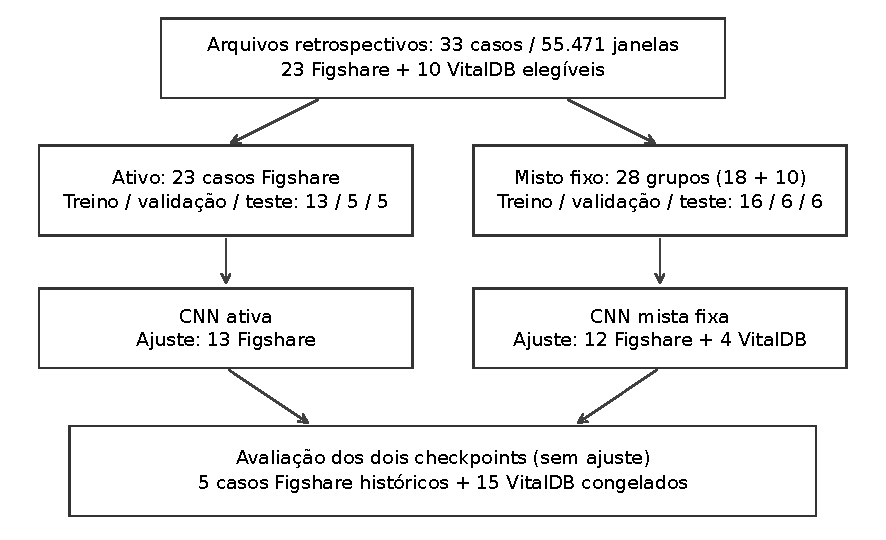
\includegraphics[width=\columnwidth]{figures/pipeline.pdf}
\caption{Fluxo retrospectivo auditável do BrainSniffer, a partir de arquivos existentes. A separação por grupo impede que janelas do mesmo grupo atravessem partições; no Figshare, o grupo é o caso. O pool elegível de 33 casos não é o corpus fixo de 28 grupos, que exclui os cinco casos históricos e se divide em 16/6/6. As setas finais indicam avaliação, nunca treino. Fontes internas \cite{brainsnifferArtefatos}; o benchmark VitalDB do misto não é confirmatório.}
\label{fig:pipeline}
\end{figure}

\section{Fundamentação e trabalhos relacionados}

O conjunto ``EEG and BIS raw data'' reúne 24 casos anônimos com EEG frontal e valores BIS, publicado no repositório Figshare sob licença CC BY 4.0 \cite{ma2017}. No mesmo corpus, um estudo anterior usou características multiescala com análise discriminante linear (Linear Discriminant Analysis, LDA); esse trabalho sustenta a descrição do corpus e das faixas, mas não é evidência de rede convolucional \cite{nsugbe2022}. Em outras configurações, uma rede estimou a concentração anestésica derivada de EEG com cadeia de aquisição dedicada, enquanto outro estudo estimou o índice de estado do paciente (Patient State Index, PSI) com quatro canais em 18 participantes idosos sedados. Esses estudos demonstram viabilidade técnica em configurações específicas, não comparabilidade direta com o rótulo, o canal ou a população do BrainSniffer \cite{park2020,shi2023}.

O VitalDB é um banco de sinais perioperatórios de milhares de cirurgias e inclui os canais de EEG e de BIS usados aqui (\texttt{BIS/EEG1\_WAV} e \texttt{BIS/BIS}) \cite{lee2022,vitaldb,clinicaldata}. O conjunto aberto (\texttt{vitaldb.net}) exige licença CC BY-NC-SA 4.0 e acordo de uso de dados, sem redistribuição. Escala, equipamento, montagem e população diferem do Figshare; por isso, o VitalDB informa a sensibilidade à troca de fonte de dados, sem isolar a causa. O conjunto DOSE-I (Zenodo, CC BY 4.0) não foi incorporado à regressão porque usa uma escala clínica de sedação por observação (Modified Observer's Assessment of Alertness/Sedation, MOAA/S) e estado de consciência, não conversíveis em BIS \cite{dosei}.

Uma reimplementação aberta do algoritmo do índice ajuda a discutir a transparência do cálculo, mas não torna um regressor treinado contra o BIS equivalente a um monitor nem certificado como tal \cite{openbis}. A independência entre desenvolvimento e avaliação, a descrição de grupos e a análise de calibração e acordo são componentes centrais de relato e avaliação de modelos; para desfecho contínuo, o tamanho da validação deve ser planejado pela precisão desejada, não pelo número de réplicas bootstrap \cite{tripodai,archer2021}.

\section{Materiais e métodos}

\subsection{Fontes, unidades de agrupamento e partições}

Cada arquivo corresponde a uma gravação inteira, tratada aqui como um caso; de cada caso são recortadas janelas de 5 s, que são as unidades de treino e de métrica. O grupo é a unidade que nunca cruza partições. O manifesto versionado \artefato{reports/corpus_manifest.json} registra 59 arquivos: 44 casos no pool de desenvolvimento e 15 casos VitalDB congelados. Os gates de qualidade são filtros aplicados antes do ajuste, que descartam casos ou janelas com problemas de escala, valores inválidos ou sinal insuficiente; após esses gates, 23 casos Figshare e dez VitalDB ficaram elegíveis, totalizando 33 casos e 55.471 janelas. O número de janelas é uma medida do volume disponível, não do desempenho, e casos longos contribuem com mais janelas do que casos curtos. No Figshare, \texttt{subject\_id} não está disponível; assim, \texttt{case\_id} evita compartilhar janelas da mesma cirurgia, mas não permite provar independência entre cirurgias de uma mesma pessoa. No VitalDB, o agrupamento usa \texttt{subjectid} e, portanto, reúne reoperações conhecidas \cite{brainsnifferArtefatos,ma2017,lee2022,clinicaldata}.

O checkpoint ativo foi desenvolvido apenas com os 23 casos Figshare elegíveis, divididos com seed 42 em 13 casos de treino, cinco de validação e cinco de teste. O candidato misto fixo excluiu desse desenvolvimento os cinco casos do holdout Figshare histórico e usou 18 grupos Figshare mais dez grupos VitalDB: 28 grupos e 49.948 janelas, com partição registrada de 16/6/6 grupos para treino, validação e teste. O ajuste usa somente 12 casos Figshare e quatro participantes VitalDB (34.792 janelas); a validação usa dois Figshare e quatro VitalDB (7.235 janelas), e o teste interno, quatro Figshare e dois VitalDB (7.921 janelas). As três partes têm papéis distintos: o treino atualiza os pesos, a validação acompanha o treinamento e apoia a parada, e só o teste interno é lido como resultado; por isso as janelas de validação não aparecem nas tabelas de desempenho. As contagens, a origem e os hashes estão em \artefato{models/brainsniffer_corpus_fixed.json}; dizer ``corpus de 28 grupos'' não significa que os 28 foram usados no ajuste \cite{brainsnifferArtefatos}.

Os mesmos cinco casos Figshare foram usados como benchmark histórico dos dois checkpoints. Para o ativo Figshare-only, os 15 casos VitalDB constituem uma avaliação cruzada de dataset. Para o misto, esses 15 participantes não entraram no ajuste, mas vêm da mesma fonte já presente no desenvolvimento; além disso, o benchmark havia sido inspecionado antes da criação do candidato. Consequentemente, ele é descrito como holdout VitalDB histórico, por participante e após exposição ao domínio, não como validação externa confirmatória. Manter o candidato fora do dashboard é uma decisão operacional: não restaura a independência de benchmarks já inspecionados, inclusive o Figshare reutilizado \cite{brainsnifferArtefatos,tripodai,imdrfn88}.

\subsection{Tarefa, pré-processamento e qualidade}

Cada exemplo é um trecho curto de EEG: 640 amostras, isto é, uma janela de 5 segundos amostrada a 128 Hz, com passo de 5 s na construção offline. Para início $t$, o alvo corresponde a $t+\mathrm{offset}$, arredondado ao intervalo do BIS do caso (5 s no Figshare e 1 s nos arquivos VitalDB normalizados). A emissão só pode ocorrer após completar a janela, aproximadamente em $t+5$ s, além do processamento; com offset zero, não se trata de previsão de um BIS futuro nem de leitura contemporânea ao fim da janela. O pipeline mantém a banda de 0,5--45 Hz, remove a interferência da rede elétrica (notch de 50 Hz) com filtro de quarta ordem e aplica a escala de amplitude registrada, com o rótulo BIS associado ao início da janela (offset padrão 0 s). O filtro usa apenas amostras passadas e presentes (estado causal), preservado por caso e entre blocos; uma rota de fase zero existe somente para análise offline explícita. Essas escolhas estão em \artefato{reports/corpus_manifest.json}, \artefato{models/brainsniffer_cnn.json} e \artefato{models/brainsniffer_corpus_fixed.json}; as fontes externas descrevem os corpora e o problema, mas não definem esta configuração \cite{brainsnifferArtefatos,ma2017,nsugbe2022}.

O controle de qualidade do corpus exige, entre outros critérios internos, pelo menos 90\% de EEG com valores numéricos válidos (finitos), lacuna inválida máxima de 2 s, qualidade global mínima 0,35, pelo menos 80\% de BIS válido e qualidade mínima 0,20 por janela. O caso Figshare 24 permanece em quarentena por escala incompatível. Esses limiares são heurísticas de engenharia ainda não calibradas para risco clínico; no replay, trechos inválidos são rejeitados antes do filtro e trechos de baixa qualidade levam o modelo a se abster. A proveniência dos limiares é exclusivamente \artefato{reports/corpus_manifest.json} \cite{brainsnifferArtefatos}.

Esse controle do corpus de desenvolvimento não se aplica aos 15 casos do benchmark VitalDB histórico. Na construção offline, \texttt{make\_windows} passa o EEG completo do caso ao pré-processador: valores inválidos (não finitos) são preenchidos por interpolação linear entre vizinhos válidos, repetindo o extremo nas bordas (vetor todo inválido vira zeros), sem limite de duração da lacuna e podendo usar amostras futuras, mesmo quando o filtro seguinte é causal. A qualidade é calculada sobre a janela bruta. O BIS inválido ou fora de $[0,100]$ é descartado, sem interpolação nessa etapa; antes, a normalização em \artefato{src/brainsniffer/data/vitaldb.py} (função \texttt{\_align\_numeric\_to\_eeg}) ordena, remove tempos duplicados e interpola os pontos BIS válidos para uma grade de 1 s apenas entre o primeiro e o último ponto válido (fora, NaN), sem limite de lacuna nem máscara persistida; aqui, válido significa finito. Como os 15 arquivos históricos contêm EEG inválido, sua avaliação offline difere da política de rejeição do replay. Esse preenchimento pode suavizar lacunas longas e limita a interpretação; política e métricas históricas foram mantidas. Descrição baseada no código e nos relatórios locais, não em recomendação dos datasets \cite{brainsnifferArtefatos}.

\subsection{Modelos e treinamento}

A rede histórica é a \texttt{Conv1DDepthEstimator}: recebe a janela de 640 amostras em um canal, é treinada com perda Smooth L1 e tem saída sigmoidal escalada para $[0,100]$. A Tabela~\ref{tab:config} explicita a arquitetura compatível em \artefato{src/brainsniffer/models/cnn.py} e os parâmetros registrados nos JSON, sem carregar pesos. Recursos posteriores do treinador e arquiteturas opcionais não são atribuídos retroativamente a esses pesos \cite{brainsnifferArtefatos}.

\begin{table}[H]
\centering
\footnotesize
\caption{Configuração histórica: JSON dos checkpoints ativo e misto fixo; arquitetura compatível no código \cite{brainsnifferArtefatos}.}
\label{tab:config}
\begin{tabular}{p{0.28\columnwidth}p{0.63\columnwidth}}
\hline
Item & Configuração registrada/compatível\\
\hline
Convolucionais (\texttt{Conv1d}) & \textit{Channels} 1--32--64--128--128; \textit{kernel} 7, 7, 5, 5; \textit{padding} 3, 3, 2, 2; \textit{stride} 1; \texttt{BatchNorm1d} + GELU\\
\textit{Pooling} e cabeça & \texttt{MaxPool1d(2)} nos 3 primeiros blocos; \texttt{AdaptiveAvgPool1d(1)}; \texttt{Linear} 128--64--1, GELU, \textit{dropout} 0,20\\
Treino (ambos) & 10 \textit{epochs}, \textit{batch} 128, \textit{lr} $10^{-3}$, \textit{wd} $10^{-4}$, \textit{seed} 42; val/teste 0,20/0,20\\
Amostragem & Misto: \textit{balanced sampling} por grupo/fonte; ativo: não registrado\\
Amplitude e \textit{notch} & \textit{Clip} $\pm100\,\mu V$, escala $50\,\mu V$, saída em $[-5,5]$; \textit{notch} 50 Hz, Q=30\\
\textit{Random Forest} & \texttt{n\_estimators}=100, \texttt{max\_depth}=12, \texttt{min\_samples\_leaf}=2, \texttt{random\_state}=42\\
\hline
\end{tabular}
\end{table}

A arquitetura compacta permite replay em CPU, mas não implica superioridade sobre redes temporais, atenção ou representações tempo-frequência \cite{brainsnifferArtefatos,park2020,shi2023}.

Como controle, o baseline extrai medidas espectrais clássicas (potência por banda, frequência de borda espectral SEF90, entropia espectral, valor eficaz RMS e \textit{line length}) e ajusta uma floresta aleatória (\textit{Random Forest}) nas mesmas janelas e partição do ativo. Detalhes em \artefato{reports/spectral_baseline_holdout.json} \cite{brainsnifferArtefatos}.

\subsection{Métricas, incerteza e análises exploratórias}

Foram calculados o erro absoluto médio (Mean Absolute Error, MAE), a raiz do erro quadrático médio (Root Mean Squared Error, RMSE), o viés e a correlação de Pearson para o rótulo contínuo, além de acurácia e macro-F1 para quatro faixas de BIS. Em leitura simples: MAE é o erro médio em pontos BIS; RMSE penaliza mais os erros grandes; viés é a diferença média predito menos referência; Pearson mede se as curvas variam juntas (associação, não acordo); macro-F1 é o acerto médio entre faixas. As métricas implementadas em \artefato{src/brainsniffer/pipeline/metrics.py} \cite{brainsnifferArtefatos} incluem MAE e RMSE, definidos por
\begin{equation}
\mathrm{MAE}=\frac{1}{n}\sum_{i=1}^{n}|y_i-\hat{y}_i|,
\qquad
\mathrm{RMSE}=\sqrt{\frac{1}{n}\sum_{i=1}^{n}(y_i-\hat{y}_i)^2}.
\end{equation}
O resultado principal agrega todas as janelas aceitas (casos longos pesam mais), em vez de tirar a média por pessoa. O viés é a média de predito menos referência. As faixas são $[0,40)$, $[40,60)$, $[60,80)$ e $[80,100]$, aqui lidas com rótulos curtos apenas para comunicação --- profunda, geral adequada, leve/transicional e acordado --- sem validar limiar clínico. Pearson quantifica associação linear e não acordo; não foram estimados, nesta execução, limites de concordância, coeficiente de concordância ou calibração clínica. As quatro faixas são apenas uma apresentação interna e não constituem classes clínicas independentes \cite{brainsnifferArtefatos,tripodai}.

A associação ordinal entre estimativa e referência é medida pela probabilidade de predição $P_K$ \cite{smith1996}, variante reescalada da medida $d_{y.x}$ de Kim: a probabilidade de o indicador ordenar corretamente duas profundidades observadas distintas, valendo 1 na ordem perfeita e 0,5 no acaso. Pares empatados na escala observada são excluídos, porque não informam ordenação, e pares empatados no indicador contam 0,5. Por depender só da ordenação, $P_K$ é invariante a reescala afim. O comando \texttt{evaluate-pk} reaproveita janelas e predições dos mesmos benchmarks, sem retreino, em \texttt{pk\_*.json} \cite{brainsnifferArtefatos,smith1996}.

O bootstrap estima a incerteza sorteando casos inteiros com reposição, juntando todas as janelas sorteadas e recalculando a métrica. Assim, respeita melhor a dependência dentro de cada caso do que sortear janelas, mas o resultado continua ponderado pela duração. Foram usadas $B=1.000$ réplicas, seed 42 e percentis 2,5/97,5 para o intervalo de 95\%. Com apenas cinco casos Figshare, o intervalo é exploratório; 1.000 réplicas não equivalem a 1.000 casos \cite{brainsnifferArtefatos,field2007,archer2021}.

A comparação VitalDB também foi calculada por caso, pareando \texttt{case\_id} e número de janelas em \artefato{reports/vitaldb_external_validation.json} e \artefato{reports/mixed_vitaldb_external.json}. A sensibilidade registrada em \artefato{reports/offset_sensitivity.json} reaplicou o checkpoint ativo aos mesmos cinco casos Figshare, sem retreino, em uma grade de $-20$ a $+20$ s. Como a grade foi examinada após o treinamento, ela formula hipótese sobre alinhamento e não escolhe o atraso do rótulo \cite{brainsnifferArtefatos,pilge2006}.

\subsection{Replay retrospectivo e trajetória ilustrativa}

Replay significa percorrer uma gravação existente, não adquirir EEG: preenche-se um buffer de 5 s e depois emite-se atualização a cada 1 s, separando valor bruto, média móvel exponencial (Exponentially Weighted Moving Average, EWMA), qualidade, instante e origem. O escopo deste TCC é exclusivamente retrospectivo, sem conexão a EEG físico. A implementação em \artefato{src/brainsniffer/pipeline/realtime.py} distingue o instante de emissão do alvo histórico no início da janela \cite{brainsnifferArtefatos}.

Para visualizar o comportamento temporal, fixou-se antes da inferência o \texttt{case19} do holdout Figshare (escolha anterior à inferência, por consistência da demonstração, não pelo desempenho), usando toda a gravação (4.355 s). O script \artefato{docs/generate_figures.py} (opção \texttt{--infer-trajectory}) reutiliza \texttt{make\_windows}, a configuração do checkpoint ativo e loader restrito, em CPU, sem treino. A curva bruta (sem EWMA) é posicionada no instante do alvo offline (início mais offset 0 s), em passos de 5 s; não representa disponibilidade sem atraso. Arrays, CSV, hashes e métricas ficam em \artefato{tmp/pdfs/trajectory-audit/}; a execução padrão não faz inferência nem download \cite{brainsnifferArtefatos}.

\section{Resultados}
\label{sec:resultados}

\subsection{Checkpoint ativo e baseline no Figshare}

No holdout Figshare do checkpoint ativo, cinco casos e 5.523 janelas produziram MAE 7,03, RMSE 11,08, viés 0,79 e Pearson 0,784. A acurácia por faixa foi 0,585 e o macro-F1 0,548. O baseline espectral, na mesma partição, obteve MAE 8,86, RMSE 13,23, Pearson 0,667, acurácia 0,540 e macro-F1 0,480. A diferença sustenta apenas vantagem da CNN nessa partição e execução, não superioridade geral. Fontes internas: \artefato{reports/figshare_holdout_evaluation.json} e \artefato{reports/spectral_baseline_holdout.json} \cite{brainsnifferArtefatos}.

\begin{table}[H]
\centering
\caption{Holdout Figshare comum: cinco casos, 5.523 janelas, seed 42; métricas agregadas por janela. Fonte interna \cite{brainsnifferArtefatos}.}
\label{tab:figshare-baseline}
\begin{tabular}{lrrrrr}
\hline
Modelo & MAE & RMSE & Pearson & Acurácia & Macro-F1\\
\hline
CNN ativa & 7,03 & 11,08 & 0,784 & 0,585 & 0,548\\
Baseline espectral & 8,86 & 13,23 & 0,667 & 0,540 & 0,480\\
\hline
\end{tabular}
\end{table}

A Figura~\ref{fig:trajectory} mostra queda inicial e elevação final em ambas as curvas, mas a CNN superestima o patamar intermediário e não reproduz várias oscilações da referência. Nas 850 janelas aceitas, MAE foi 8,72, RMSE 10,21, viés $+4{,}79$ pontos BIS e Pearson 0,910: associação alta não elimina erro sistemático. É um exemplo ilustrativo, não evidência de generalização. A série BIS tem 906 pontos e se estende além do EEG; das 871 janelas completas, 21 foram rejeitadas, e 35 pontos finais não têm janela correspondente. As 56 posições sem previsão permanecem NaN; não havia EEG inválido neste caso. Fonte: auditoria em \artefato{tmp/pdfs/trajectory-audit/case19.json} \cite{brainsnifferArtefatos}.

\begin{figure}[tbp]
\centering
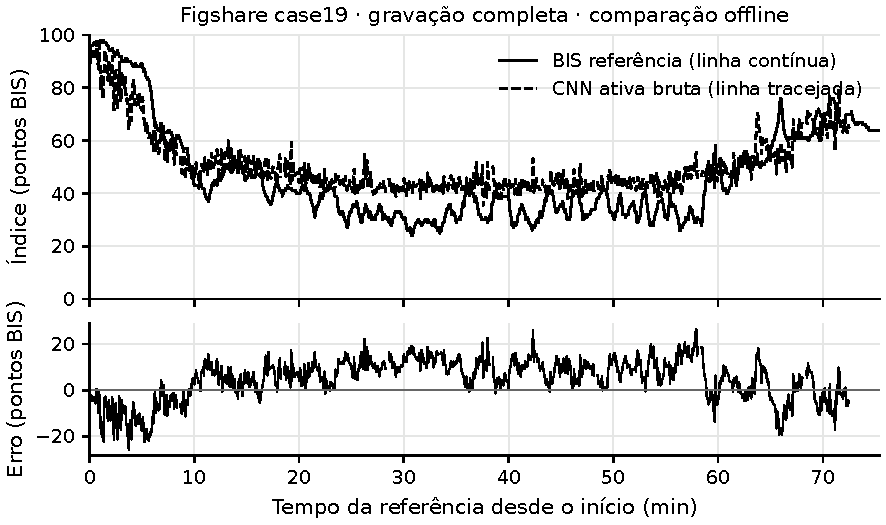
\includegraphics[width=\columnwidth]{figures/bis_trajectory.pdf}
\caption{Trajetória offline do Figshare \texttt{case19}, fixado antes da inferência por consistência da demonstração, não por desempenho. BIS original e CNN ativa bruta (sem EWMA), com erro no painel inferior. Alvo no início da janela (offset 0 s), não no instante de emissão. Lacunas preservadas; a cauda BIS excede o suporte EEG. Fontes: \artefato{data/raw/case19.mat} e auditoria \artefato{tmp/pdfs/trajectory-audit/case19.json}. Exemplo individual \cite{brainsnifferArtefatos}.}
\label{fig:trajectory}
\end{figure}

\subsection{Comparação dos checkpoints nos benchmarks históricos}

O candidato misto apresentou MAE 6,69, RMSE 10,67, viés 2,12, Pearson 0,818 e macro-F1 0,574 no holdout Figshare. Nos 15 participantes e 38.730 janelas do holdout VitalDB histórico, obteve 8,60, 11,74, $-1{,}01$, 0,688 e 0,486. O ativo obteve, respectivamente, 7,03/11,08/0,79/0,784/0,548 no Figshare e 12,43/18,80/1,40/0,024/0,398 no VitalDB. Os valores vêm de \artefato{reports/figshare_holdout_evaluation.json}, \artefato{reports/mixed_fixed_figshare_holdout.json}, \artefato{reports/vitaldb_external_validation.json} e \artefato{reports/mixed_vitaldb_external.json} \cite{brainsnifferArtefatos}.

\begin{table}[H]
\centering
\caption{Comparação retrospectiva nos mesmos benchmarks históricos. ``Visto'' indica fonte vista no desenvolvimento. Fonte interna \cite{brainsnifferArtefatos}.}
\label{tab:benchmarks}
\begin{tabular}{llcrrr}
\hline
Benchmark & Modelo (fontes vistas) & Casos & MAE & RMSE & Pearson\\
\hline
Figshare & ativo (Figshare) & 5 & 7,03 & 11,08 & 0,784\\
Figshare & misto (Figshare+VitalDB) & 5 & 6,69 & 10,67 & 0,818\\
VitalDB & ativo (Figshare) & 15 & 12,43 & 18,80 & 0,024\\
VitalDB & misto (Figshare+VitalDB) & 15 & 8,60 & 11,74 & 0,688\\
\hline
\end{tabular}
\end{table}

No VitalDB, o MAE do candidato caiu em 14 dos 15 casos pareados; no \texttt{vitaldb\_case16}, subiu cerca de 0,67 ponto BIS. Na Figura~\ref{fig:comparison}c, cada linha é um caso, ordenado pela diferença misto menos ativo, e os dois pontos são os MAE de cada modelo no mesmo caso; uma linha apontando para a esquerda indica que o misto errou menos. A leitura é pareada de propósito: comparar médias agregadas de modelos diferentes poderia esconder que eles acertam os mesmos casos ou que um grupo pequeno de casos longos domina a média. O painel (a) e o (b) mostram os agregados, mas é o painel (c) que revela a heterogeneidade: o ganho não é uniforme, e 14 acertos contra 1 piora convivem com casos em que a margem é pequena. Como os agregados são calculados por janela, casos longos pesam mais do que casos curtos, e a média pode não corresponder à de um caso típico. Essa comparação descreve adaptação após exposição ao VitalDB, não transporte para nova fonte \cite{brainsnifferArtefatos}.

\begin{figure}[tbp]
\centering
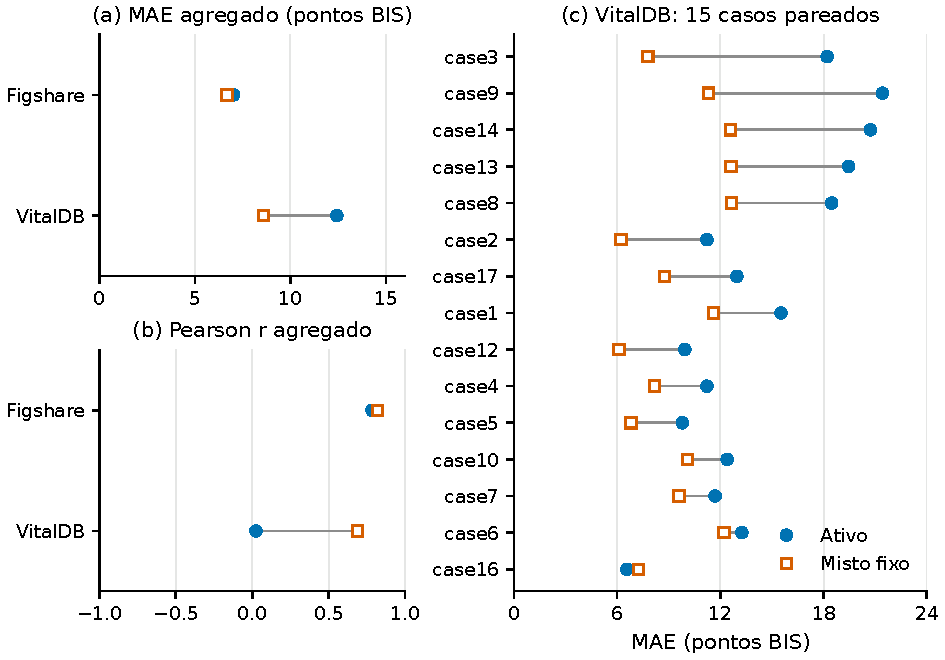
\includegraphics[width=\columnwidth]{figures/comparison.pdf}
\caption{Agregados por janela no Figshare (5 casos/5.523 janelas) e VitalDB (15/38.730) e MAE pareado por caso, ordenado pela diferença misto menos ativo. O ativo viu só o Figshare; o misto já viu outros participantes VitalDB. Pontos e linhas vêm dos quatro relatórios citados no texto; 14/15 casos melhoram, mas o caso 16 piora cerca de 0,67 \cite{brainsnifferArtefatos}.}
\label{fig:comparison}
\end{figure}

\subsection{Probabilidade de predição $P_K$}

A associação ordinal é medida nos dois benchmarks pela probabilidade de predição $P_K$ de Smith, Dutton e Smith \cite{smith1996}, que responde a uma pergunta diferente da de MAE e viés: com que frequência o indicador ordena corretamente duas profundidades observadas distintas? A Tabela~\ref{tab:pk} e a Figura~\ref{fig:pk} trazem os valores e os intervalos por caso. Fontes: os quatro relatórios \texttt{pk\_*.json} em \artefato{reports/} \cite{brainsnifferArtefatos}.

\begin{table}[H]
\centering
\small
\caption{Probabilidade de predição $P_K$ nos mesmos benchmarks históricos. $P_K=1$ é ordem perfeita e $0{,}5$ é acaso. IC 95\% por reamostragem de casos ($B=1.000$, seed 42). MAE e Pearson repetem as tabelas anteriores.}
\label{tab:pk}
\begin{tabular}{llrrrrr}
\hline
Benchmark & Modelo & Janelas & $P_K$ & IC 95\% & MAE & Pearson\\
\hline
Figshare & ativo & 5.523 & 0,773 & 0,679--0,828 & 7,03 & 0,784\\
Figshare & misto & 5.523 & 0,774 & 0,676--0,835 & 6,69 & 0,818\\
VitalDB & ativo & 38.730 & 0,515 & 0,434--0,581 & 12,43 & 0,024\\
VitalDB & misto & 38.730 & 0,672 & 0,591--0,737 & 8,60 & 0,688\\
\hline
\end{tabular}
\end{table}

No Figshare, o ativo obtém $P_K$ 0,773 (0,679--0,828) e o misto 0,774 (0,676--0,835). O achado desta seção está na leitura conjunta com a Tabela~\ref{tab:benchmarks}: o misto melhora MAE (7,03 para 6,69) e Pearson (0,784 para 0,818), mas mantém $P_K$ praticamente idêntico, ou seja, o ganho é de escala e não de ordenação. No VitalDB, o ativo tem $P_K$ 0,515 (0,434--0,581), indistinguível do acaso, e o misto 0,672 (0,591--0,737). Como $P_K$ ignora erro sistemático, ele separa duas leituras que o MAE confunde \cite{smith1996,brainsnifferArtefatos}.

\begin{figure}[tbp]
\centering
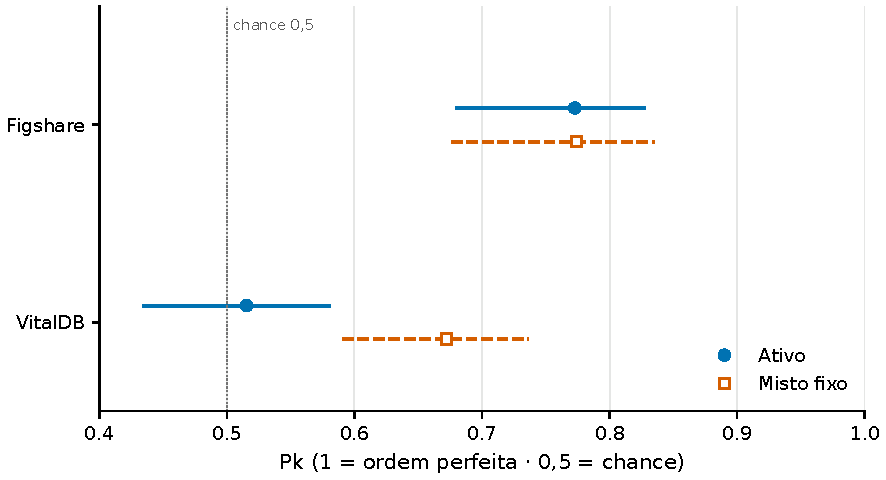
\includegraphics[width=0.86\columnwidth]{figures/pk_prediction.pdf}
\caption{Probabilidade de predição $P_K$ (Figshare 5/5.523; VitalDB 15/38.730), ativo vs misto, com IC 95\% por reamostragem de casos ($B=1.000$, seed 42). A linha pontilhada marca o acaso em 0,5. O indicador é a estimativa da CNN e a escala observada é o BIS de referência do monitor, não um desfecho de resposta ao estímulo \cite{smith1996,brainsnifferArtefatos}.}
\label{fig:pk}
\end{figure}


\subsection{Bootstrap agrupado e sensibilidade ao offset}

No Figshare, o ativo apresentou MAE observado 7,03 (IC percentil 95\%: 6,38--8,24) e Pearson 0,784 (0,703--0,881); para o misto, os valores foram 6,69 (5,65--8,53) e 0,818 (0,751--0,890). No VitalDB, o ativo apresentou 12,43 (11,05--14,45) e 0,024 ($-0{,}126$--0,193), enquanto o misto apresentou 8,60 (7,57--9,95) e 0,688 (0,606--0,752). Os marcadores da Figura~\ref{fig:bootstrap} são essas métricas observadas; somente as barras representam os intervalos das réplicas. As médias das réplicas bootstrap não substituem esses pontos observados. Os mesmos quatro relatórios registram $B$, seed, unidade e intervalos \cite{brainsnifferArtefatos}.

\begin{figure}[tbp]
\centering
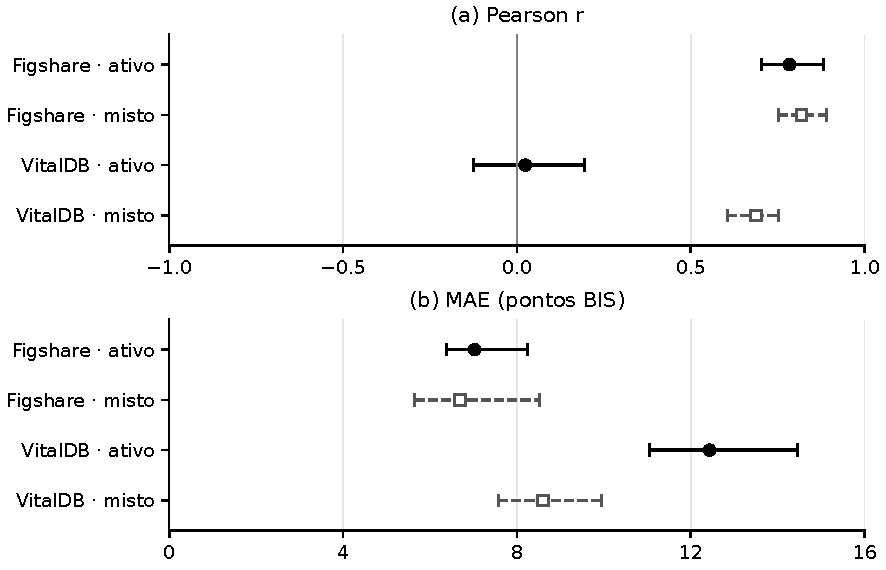
\includegraphics[width=\columnwidth]{figures/bootstrap_intervals.pdf}
\caption{Métricas observadas (marcadores) e intervalos percentis de 95\% (barras) do bootstrap por caso ($B=1.000$, seed 42). Cada caso sorteado contribui com todas as janelas. O $n=5$ do Figshare limita a leitura \cite{brainsnifferArtefatos}.}
\label{fig:bootstrap}
\end{figure}

Na grade de offset, o ativo variou de MAE 7,22/Pearson 0,766 em $-20$ s para 7,03/0,784 em 0 s e 6,76/0,799 em $+20$ s. Um offset positivo associa a janela EEG a um BIS posterior. A tendência foi observada pós-hoc, sem retreino, e não identifica causalmente atraso do monitor nem autoriza mudar o offset padrão. Fonte interna: \artefato{reports/offset_sensitivity.json} \cite{brainsnifferArtefatos}; contexto sobre atraso de índices processados em \cite{pilge2006}.

\begin{figure}[tbp]
\centering
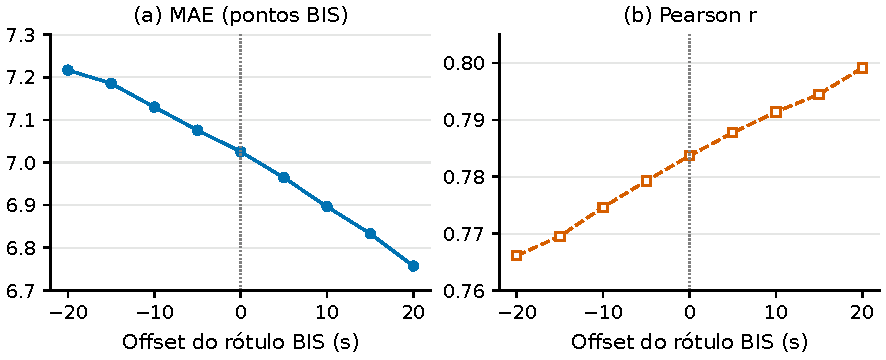
\includegraphics[width=\columnwidth]{figures/offset_sensitivity.pdf}
\caption{Sensibilidade pós-hoc ao alinhamento do rótulo em cinco casos Figshare. O número de janelas varia de 5.503 a 5.525, sem restrição a suporte comum. A linha vertical indica o padrão 0 s. A análise sem retreino gera hipótese e não seleciona atraso. Fonte: \artefato{reports/offset_sensitivity.json} \cite{brainsnifferArtefatos}.}
\label{fig:offset}
\end{figure}

\FloatBarrier
\subsection{Painéis de apoio: corpus, qualidade e projeção}

As duas figuras seguintes detalham o que as tabelas e os agregados comprimem. A primeira caracteriza o corpus que alimenta o protótipo; a segunda documenta o comportamento do treinamento e uma projeção declarada de planejamento. Os painéis de composição e de qualidade da Figura~\ref{fig:corpus} e o histórico da Figura~\ref{fig:training}a são leituras diretas de \artefato{reports/corpus\_manifest.json} e \artefato{models/brainsniffer\_cnn.json}; somente a projeção da Figura~\ref{fig:training}b é cenário ancorado no MAE 7,03 medido, não curva observada \cite{brainsnifferArtefatos}.

A Figura~\ref{fig:corpus}a separa os casos por fonte em três estados mutuamente exclusivos. ``Elegível'' é o caso que passou por todos os gates de qualidade e entrou no pool de desenvolvimento; ``quarentena'' é o caso retido por falha de gate, como o Figshare 24, cuja escala de amplitude é incompatível; ``benchmark histórico'' é o caso reservado para avaliação, que não ajusta nenhum checkpoint. A leitura correta é de composição, não de desempenho: barras maiores não indicam melhor qualidade. A Figura~\ref{fig:corpus}b cruza a fração de amostras de EEG finitas (eixo horizontal) com a fração de janelas aceitas (eixo vertical) e mostra por que os dois gates não são redundantes. Um caso pode ter quase todo o EEG finito e ainda perder janelas por qualidade de sinal insuficiente; outro pode ter lacunas inválidas e ser retido antes da contagem. A linha tracejada marca o gate de 90\% de amostras finitas; pontos à sua esquerda foram retidos independentemente do eixo vertical \cite{brainsnifferArtefatos}.

\begin{figure}[tbp]
\centering
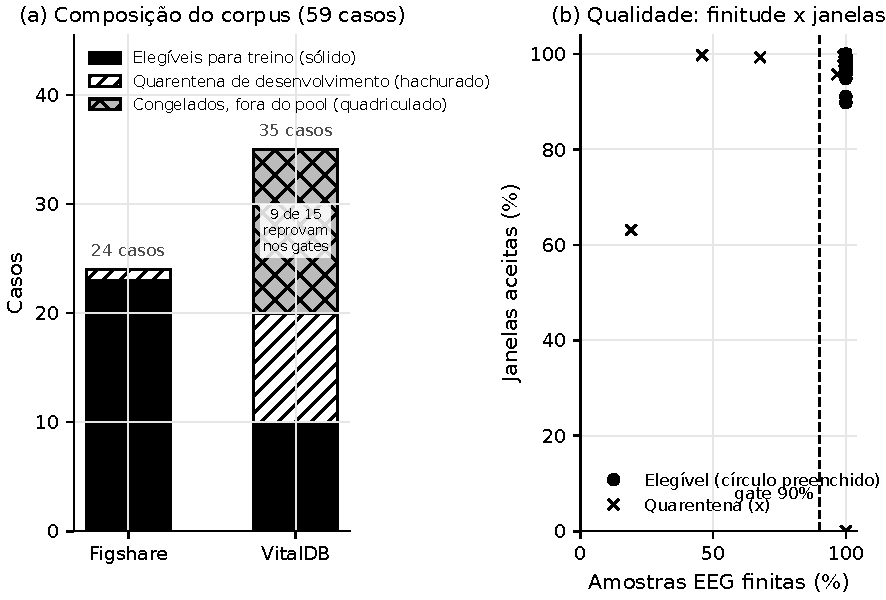
\includegraphics[width=\columnwidth]{figures/corpus_panels.pdf}
\caption{Composição e qualidade do corpus de desenvolvimento. (a) Casos por fonte, separando elegíveis, quarentena e benchmark histórico; a soma rotulada é o total de arquivos da fonte. (b) Fração de amostras de EEG finitas contra fração de janelas aceitas; a linha tracejada marca o gate de 90\% de finitude. Gates e contagens vêm de \artefato{reports/corpus\_manifest.json} \cite{brainsnifferArtefatos}.}
\label{fig:corpus}
\end{figure}

A Figura~\ref{fig:training}a acompanha a perda de treino e as métricas de validação por época. As duas curvas medem coisas diferentes: a perda de treino é a função otimizada (Smooth L1, adimensional, na escala normalizada) e tende a cair de forma monotônica, enquanto MAE e RMSE de validação são medidas em pontos BIS e podem oscilar por variação de amostragem entre épocas. Por isso, o critério de leitura é a validação, não a perda de treino; separadamente, a validação também serve para detectar sobreajuste, que apareceria como queda da perda de treino com piora simultânea do MAE de validação. Nesta execução as três curvas ficam estáveis após poucas épocas, o que é consistente com o teto fixo de dez épocas adotado no protocolo. A Figura~\ref{fig:training}b projeta o MAE para contagens maiores de casos de treino por uma curva teórica ancorada no único ponto medido (13 casos de treino, MAE 7,03). O eixo horizontal é logarítmico porque o ganho por caso é decrescente; a curva não foi ajustada a dados novos, não substitui o holdout e serve apenas para dimensionar uma coleta futura \cite{brainsnifferArtefatos,archer2021}.

\begin{figure}[tbp]
\centering
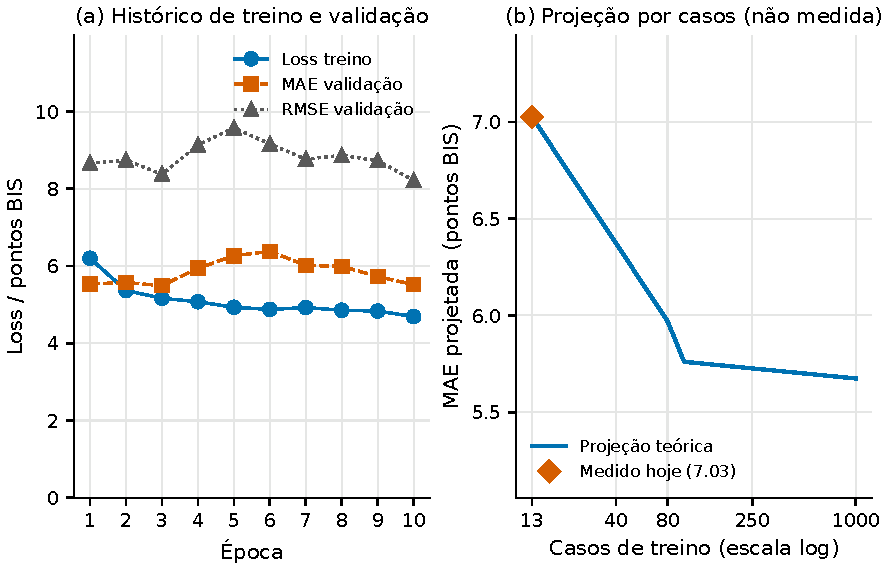
\includegraphics[width=\columnwidth]{figures/training_panels.pdf}
\caption{Apoio de treinamento e planejamento. (a) Histórico de treino e validação do checkpoint ativo por época: perda de treino (adimensional) e MAE/RMSE de validação (pontos BIS). (b) Projeção teórica de MAE por número de casos de treino, em escala logarítmica, ancorada no único valor medido (13 casos, MAE 7,03): cenário de planejamento, não curva medida \cite{brainsnifferArtefatos}.}
\label{fig:training}
\end{figure}


\section{Discussão e limitações}

A degradação do ativo treinado só no Figshare, quando aplicado ao VitalDB, é evidência interna de sensibilidade à troca de fonte de dados, não prova de qual diferença (equipamento, centro, ganho, montagem, população ou distribuição do BIS) a causou. A redução de erro do candidato misto é compatível com adaptação após incorporar participantes VitalDB ao desenvolvimento; como esse benchmark é da mesma fonte e já havia sido observado, ele deve gerar uma hipótese para uma nova coorte travada, não uma alegação de generalização externa \cite{brainsnifferArtefatos,lee2022,tripodai,imdrfn88}.

A melhora em 14/15 casos coexiste com piora no caso 16, e os agregados por janela privilegiam cirurgias longas. Além disso, Pearson pode aumentar mesmo com viés ou discordância relevantes. Métricas por participante e análises de acordo/calibração são extensões possíveis, não resultados já demonstrados \cite{brainsnifferArtefatos,tripodai,archer2021}.

O bootstrap representa somente a variabilidade de reamostrar os casos disponíveis sob o algoritmo escolhido. Ele não cobre incerteza de treinamento, seleção de checkpoint, hiperparâmetros, mudança de centro ou erro do próprio rótulo BIS. O pequeno $n$ Figshare e o reaproveitamento do benchmark VitalDB impedem leitura confirmatória \cite{brainsnifferArtefatos,field2007,archer2021}.

O alvo é a saída BIS, que pode responder a EMG, bloqueio neuromuscular, cetamina e atrasos; portanto, baixo erro contra o monitor não equivale a medir consciência ou efeito farmacológico verdadeiro \cite{schuller2015,hans2005,pilge2006}. De modo semelhante, as faixas e os limiares de qualidade do protótipo são heurísticas internas \cite{brainsnifferArtefatos}. DOSE-I deve permanecer uma tarefa separada para MOAA/S e estado de consciência, sem conversão artificial para BIS \cite{dosei}.

A leitura ordinal separa dois diagnósticos que o MAE confunde: no VitalDB o ativo tem $P_K$ 0,515, praticamente acaso, enquanto no Figshare alcança 0,773; o modelo não perdeu apenas calibração, perdeu a capacidade de ordenar profundidade. No Figshare, o misto eleva Pearson sem mover $P_K$, o que distingue ajuste de escala de ganho de ordenação. Como a escala observada aqui é o BIS de referência, e não um desfecho de resposta ao estímulo, esses valores não substituem validação clínica \cite{smith1996,brainsnifferArtefatos}.

Em engenharia, a cadeia registra hashes, partições, pré-processamento, relatórios e replay de arquivos. A trajetória individual torna visíveis erros que os agregados ocultam, mas não substitui a análise entre casos. Investigar o efeito das lacunas e a concordância em dados secundários são extensões metodológicas possíveis, não requisitos adicionais para concluir este TCC retrospectivo \cite{brainsnifferArtefatos,tripodai}.

\section{Conclusão}

O BrainSniffer entrega um protótipo aberto e reproduzível para estimar uma referência BIS a partir de EEG frontal em arquivos e replay retrospectivo. Como sintetizado na Seção~\ref{sec:resultados}, o checkpoint ativo mostrou desempenho interno melhor que o baseline espectral, mas perdeu associação no VitalDB; o candidato misto reduziu o erro após exposição a esse domínio, com heterogeneidade por caso e sem independência confirmatória. Os resultados são retrospectivos, exploratórios e limitados pelo rótulo, pelo número de casos, pelo reuso dos benchmarks e pelas políticas de imputação offline \cite{brainsnifferArtefatos}.

A contribuição defensável é uma base auditável para formular e testar hipóteses, não um sistema clínico. O software não mede consciência, não prescreve dose, não controla bomba e não deve acionar alarme ou conduta. O TCC se encerra com a implementação documentada, a comparação existente e a explicitação dos limites; uma futura alegação de generalização exigiria avaliação independente \cite{brainsnifferArtefatos,tripodai}.

\subsection*{Ética, governança e conformidade}

Esta etapa usa os corpora secundários Figshare e VitalDB, cujas publicações e páginas oficiais identificam a origem dos dados, não a aprovação institucional deste projeto \cite{ma2017,lee2022,clinicaldata}. Não se relata coleta prospectiva nem intervenção. Não foi apresentado aqui número de parecer, aprovação ou dispensa institucional, e nenhum é presumido a partir da disponibilidade dos dados. Os termos de uso e o enquadramento ético devem ser confirmados pelo autor e pela instituição, conforme os procedimentos institucionais aplicáveis, antes de qualquer estudo futuro. A nova inferência ilustrativa em um caso não reexecuta o treinamento nem os benchmarks completos; a compilação não valida alterações simultâneas do sistema.

\bibliographystyle{sbc}
\bibliography{referencias}

\end{document}
